\documentclass[tikz,border=10pt]{standalone}
\begin{document}
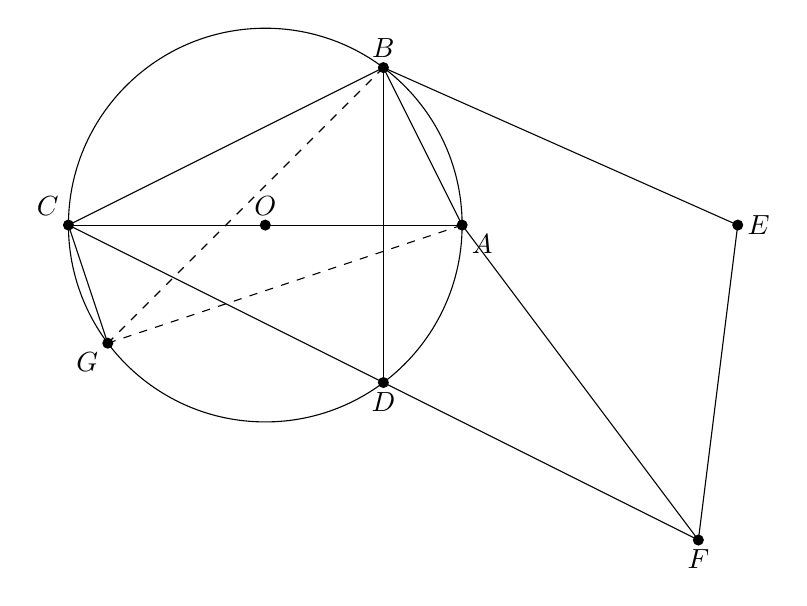
\begin{tikzpicture}
    % Define coordinates
    \coordinate (O) at (0,0);
    \coordinate (C) at (-2.5, 0);
    \coordinate (A) at (2.5, 0);
    \coordinate (E) at (6, 0);
    \coordinate (B) at (1.5, 2);
    \coordinate (D) at (1.5, -2);
    \coordinate (G) at (-2, -1.5);
    \coordinate (F) at (5.5, -4);

    % Draw Circle
    \draw (O) circle (2.5);

    % Draw solid lines
    \draw (C) -- (A); % Diameter CA
    \draw (B) -- (D); % Chord BD
    \draw (B) -- (C);
    \draw (B) -- (A);
    \draw (C) -- (F); % Line CDF
    \draw (A) -- (F);
    \draw (E) -- (F);
    \draw (B) -- (E);
    \draw (C) -- (G); % Chord CG

    % Draw dashed lines
    \draw[dashed] (B) -- (G);
    \draw[dashed] (A) -- (G);

    % Draw Points
    \fill (O) circle (2pt);
    \fill (A) circle (2pt);
    \fill (B) circle (2pt);
    \fill (C) circle (2pt);
    \fill (D) circle (2pt);
    \fill (E) circle (2pt);
    \fill (F) circle (2pt);
    \fill (G) circle (2pt);

    % Labels
    \node[above left] at (C) {$C$};
    \node[above] at (B) {$B$};
    \node[below] at (D) {$D$};
    \node[above] at (O) {$O$};
    \node[below right] at (A) {$A$};
    \node[right] at (E) {$E$};
    \node[below] at (F) {$F$};
    \node[below left] at (G) {$G$};
\end{tikzpicture}
\end{document}
